\documentclass{article}
\usepackage{tikz}
\usetikzlibrary{fit}

\tikzset{
  explored/.style = {circle, fill=gray, draw=black, very thick},
  discovered/.style = {circle, draw=black},
  neutral/.style = {circle, dashed, draw=black}
}

\begin{document}
\begin{figure}
\centering
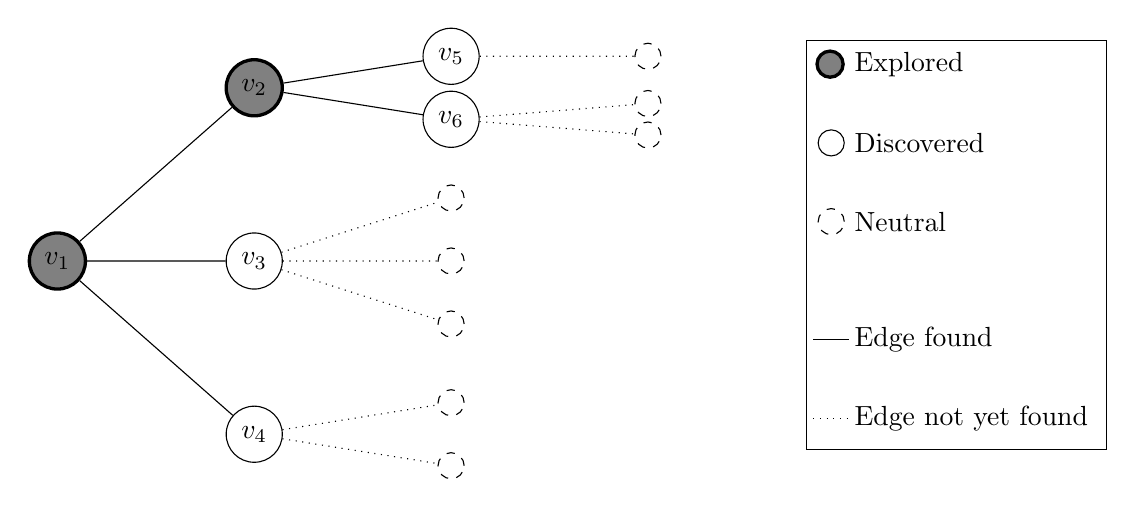
\begin{tikzpicture}[level distance = 25mm, scale = 1]
% GRAPH
\tikzstyle{level 1}=[sibling distance=22mm]
\tikzstyle{level 2}=[sibling distance=8mm]
\tikzstyle{level 3}=[sibling distance=4mm]
\node (A) [explored] {$v_1$} [grow=right]
	child { node [discovered] {$v_4$}
		child { node [neutral] {}
			edge from parent [dotted]}
		child { node [neutral] {}
			edge from parent [dotted]}
	}
	child { node [discovered] {$v_3$}
		child { node [neutral] {}
			edge from parent [dotted]}
		child { node [neutral] {}
			edge from parent [dotted]}
		child { node [neutral] {}
			edge from parent [dotted]}
	}
	child { node [explored] {$v_2$}
		child { node [discovered] {$v_6$}
			child { node [neutral] {}
				edge from parent [dotted]}
			child { node [neutral] {}
				edge from parent [dotted]}}
		child { node [discovered] {$v_5$}
			child { node [neutral] {}
				edge from parent [dotted]}}
	}
;
% LEGEND NODES
\node [explored, anchor=east](Legend-E-Node) at (10,2.5){};  
\node[anchor=west](Legend-E-Text) at (10,2.5){Explored}; 
\node [discovered, anchor=east](Legend-D-Node) at (10,1.5){};  
\node[anchor=west](Legend-D-Text) at (10,1.5){Discovered}; 
\node [neutral, anchor=east](Legend-N-Node) at (10,0.5){};  
\node[anchor=west](Legend-N-Text) at (10,0.5){Neutral}; 
% LEGEND LINES
\draw (9.6,-1) -- (10.05,-1); 
\node[anchor=west](Legend-F-Text) at (10,-1){Edge found}; 
\draw [dotted] (9.6,-2) -- (10.05,-2); 
\node[anchor=west](Legend-NF-Text) at (10,-2){Edge not yet found}; 
% LEGEND BOX
\node[draw,fit=(Legend-E-Node)(Legend-N-Text)(Legend-D-Text)(Legend-NF-Text)] {};
\end{tikzpicture}
\caption{Discovering nodes}
\end{figure}
\end{document}